\documentclass[a4paper,10pt,twocolumn]{jsarticle}
\usepackage{myjlababsstyle}
\begin{document}
\section{実験}
\subsection{方法}
本研究の印象推定方法によって推定された歌詞と歌詞中に出現するフレーズの印象が妥当であるか効果を評価する.
実験参加者は10代後半から20代前半の大学生男女11名である.男女の内訳は男子7名,女子4名である.
実験参加者には実験前に印象の定義について十分に説明をした.

アンケートを作成しデータを収集した.歌詞とフレーズに対して喜怒哀楽いずれの感性を感じるか質問した.
質問の解答項目は喜・怒・哀・楽・わからないである.
アンケートに使用した歌詞とフレーズは4印象のグループからそれぞれ原点からの距離に基づいてward法で3つのグループにクラスタリングをしたものから1つずつランダムで選出した.

\subsection{結果}
推定した印象と実験参加者の回答の過半数以上が合っていることを妥当であると定義する.
歌詞においては喜のクラスの印象の推定結果が妥当であることを確認した.
フレーズにおいては喜のクラスと哀,楽のクラスの1部分において妥当であることを確認した.妥当であると判断したグループ数を印象ごとに図1で示す.
\begin{figure}[b]
    \centering
    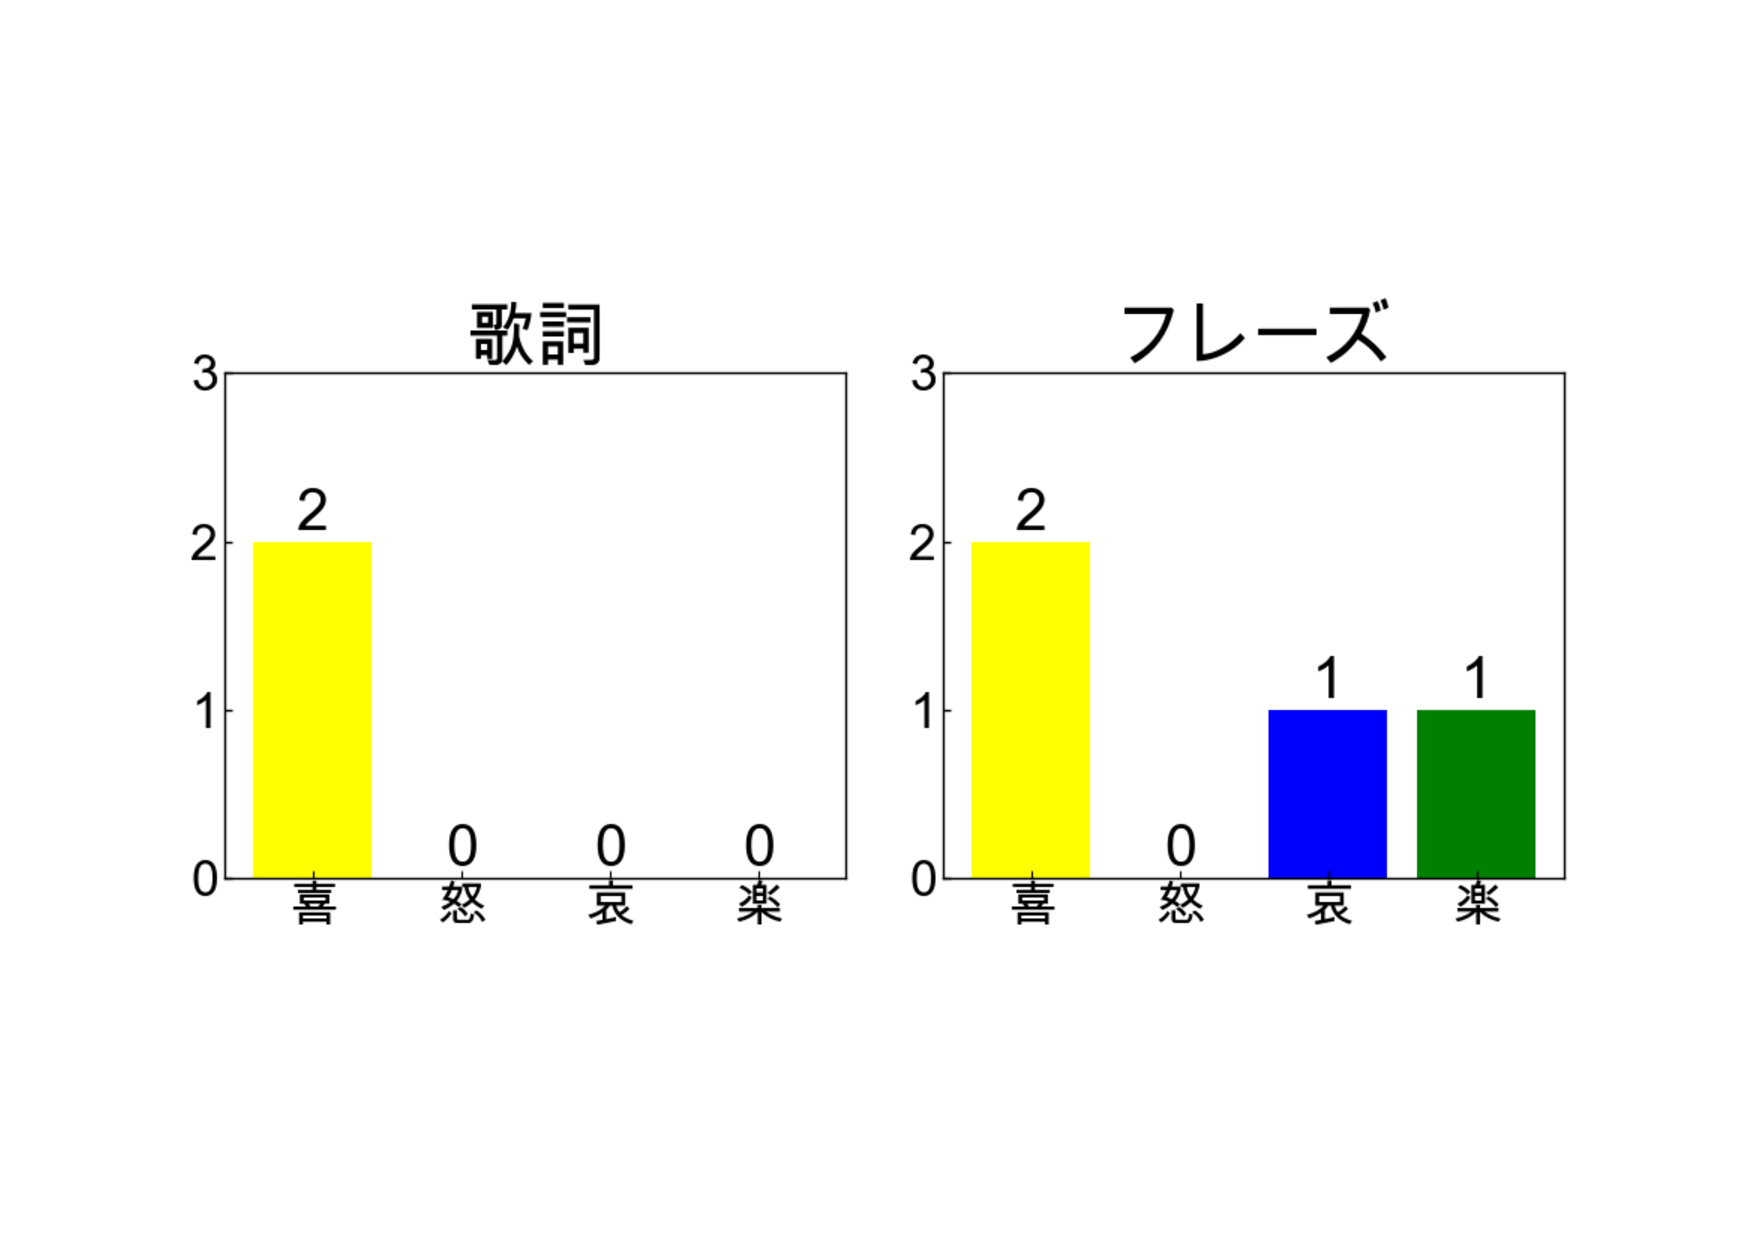
\includegraphics[angle=-90,width=8cm]{result.pdf}
    \vspace{0mm}
    \caption{妥当であると判断されたグループ数}
    \label{fig:mms}
    \vspace{5mm}
\end{figure}
\subsection{考察}
歌詞とフレーズどちらにおいても喜の印象の推定結果が妥当であった理由は事前知識が他の印象と比べて豊富であったためであると考えられる.
事前知識が十分に収集できないとMAP推定する際に未知の単語が多くなる.
未知の単語に対してMAP推定する際には無情報事前分布を与えるので,MAP推定前のP(w\verb+|+z)がMAP推定後のP(w\verb+|+z)の分布に大きく影響を残す.
したがって潜在的トピックを印象に制限できないため妥当でない結果となったと考える.

%
\end{document}
